\documentclass[1p]{elsarticle_modified}
%\bibliographystyle{elsarticle-num}

%\usepackage[colorlinks]{hyperref}
%\usepackage{abbrmath_seonhwa} %\Abb, \Ascr, \Acal ,\Abf, \Afrak
\usepackage{amsfonts}
\usepackage{amssymb}
\usepackage{amsmath}
\usepackage{amsthm}
\usepackage{scalefnt}
\usepackage{amsbsy}
\usepackage{kotex}
\usepackage{caption}
\usepackage{subfig}
\usepackage{color}
\usepackage{graphicx}
\usepackage{xcolor} %% white, black, red, green, blue, cyan, magenta, yellow
\usepackage{float}
\usepackage{setspace}
\usepackage{hyperref}

\usepackage{tikz}
\usetikzlibrary{arrows}

\usepackage{multirow}
\usepackage{array} % fixed length table
\usepackage{hhline}

%%%%%%%%%%%%%%%%%%%%%
\makeatletter
\renewcommand*\env@matrix[1][\arraystretch]{%
	\edef\arraystretch{#1}%
	\hskip -\arraycolsep
	\let\@ifnextchar\new@ifnextchar
	\array{*\c@MaxMatrixCols c}}
\makeatother %https://tex.stackexchange.com/questions/14071/how-can-i-increase-the-line-spacing-in-a-matrix
%%%%%%%%%%%%%%%

\usepackage[normalem]{ulem}

\newcommand{\msout}[1]{\ifmmode\text{\sout{\ensuremath{#1}}}\else\sout{#1}\fi}
%SOURCE: \msout is \stkout macro in https://tex.stackexchange.com/questions/20609/strikeout-in-math-mode

\newcommand{\cancel}[1]{
	\ifmmode
	{\color{red}\msout{#1}}
	\else
	{\color{red}\sout{#1}}
	\fi
}

\newcommand{\add}[1]{
	{\color{blue}\uwave{#1}}
}

\newcommand{\replace}[2]{
	\ifmmode
	{\color{red}\msout{#1}}{\color{blue}\uwave{#2}}
	\else
	{\color{red}\sout{#1}}{\color{blue}\uwave{#2}}
	\fi
}

\newcommand{\Sol}{\mathcal{S}} %segment
\newcommand{\D}{D} %diagram
\newcommand{\A}{\mathcal{A}} %arc


%%%%%%%%%%%%%%%%%%%%%%%%%%%%%5 test

\def\sl{\operatorname{\textup{SL}}(2,\Cbb)}
\def\psl{\operatorname{\textup{PSL}}(2,\Cbb)}
\def\quan{\mkern 1mu \triangleright \mkern 1mu}

\theoremstyle{definition}
\newtheorem{thm}{Theorem}[section]
\newtheorem{prop}[thm]{Proposition}
\newtheorem{lem}[thm]{Lemma}
\newtheorem{ques}[thm]{Question}
\newtheorem{cor}[thm]{Corollary}
\newtheorem{defn}[thm]{Definition}
\newtheorem{exam}[thm]{Example}
\newtheorem{rmk}[thm]{Remark}
\newtheorem{alg}[thm]{Algorithm}

\newcommand{\I}{\sqrt{-1}}
\begin{document}

%\begin{frontmatter}
%
%\title{Boundary parabolic representations of knots up to 8 crossings}
%
%%% Group authors per affiliation:
%\author{Yunhi Cho} 
%\address{Department of Mathematics, University of Seoul, Seoul, Korea}
%\ead{yhcho@uos.ac.kr}
%
%
%\author{Seonhwa Kim} %\fnref{s_kim}}
%\address{Center for Geometry and Physics, Institute for Basic Science, Pohang, 37673, Korea}
%\ead{ryeona17@ibs.re.kr}
%
%\author{Hyuk Kim}
%\address{Department of Mathematical Sciences, Seoul National University, Seoul 08826, Korea}
%\ead{hyukkim@snu.ac.kr}
%
%\author{Seokbeom Yoon}
%\address{Department of Mathematical Sciences, Seoul National University, Seoul, 08826,  Korea}
%\ead{sbyoon15@snu.ac.kr}
%
%\begin{abstract}
%We find all boundary parabolic representation of knots up to 8 crossings.
%
%\end{abstract}
%\begin{keyword}
%    \MSC[2010] 57M25 
%\end{keyword}
%
%\end{frontmatter}

%\linenumbers
%\tableofcontents
%
\newcommand\colored[1]{\textcolor{white}{\rule[-0.35ex]{0.8em}{1.4ex}}\kern-0.8em\color{red} #1}%
%\newcommand\colored[1]{\textcolor{white}{ #1}\kern-2.17ex	\textcolor{white}{ #1}\kern-1.81ex	\textcolor{white}{ #1}\kern-2.15ex\color{red}#1	}

{\Large $\underline{12a_{0193}~(K12a_{0193})}$}

\setlength{\tabcolsep}{10pt}
\renewcommand{\arraystretch}{1.6}
\vspace{1cm}\begin{tabular}{m{100pt}>{\centering\arraybackslash}m{274pt}}
\multirow{5}{120pt}{
	\centering
	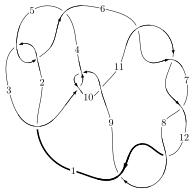
\includegraphics[width=112pt]{../../../GIT/diagram.site/Diagrams/png/994_12a_0193.png}\\
\ \ \ A knot diagram\footnotemark}&
\allowdisplaybreaks
\textbf{Linearized knot diagam} \\
\cline{2-2}
 &
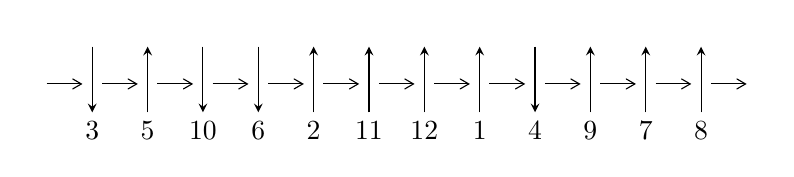
\begin{tikzpicture}[x=20pt, y=17pt]
	% nodes
	\node (C0) at (0, 0) {};
	\node (C1) at (1, 0) {};
	\node (C1U) at (1, +1) {};
	\node (C1D) at (1, -1) {3};

	\node (C2) at (2, 0) {};
	\node (C2U) at (2, +1) {};
	\node (C2D) at (2, -1) {5};

	\node (C3) at (3, 0) {};
	\node (C3U) at (3, +1) {};
	\node (C3D) at (3, -1) {10};

	\node (C4) at (4, 0) {};
	\node (C4U) at (4, +1) {};
	\node (C4D) at (4, -1) {6};

	\node (C5) at (5, 0) {};
	\node (C5U) at (5, +1) {};
	\node (C5D) at (5, -1) {2};

	\node (C6) at (6, 0) {};
	\node (C6U) at (6, +1) {};
	\node (C6D) at (6, -1) {11};

	\node (C7) at (7, 0) {};
	\node (C7U) at (7, +1) {};
	\node (C7D) at (7, -1) {12};

	\node (C8) at (8, 0) {};
	\node (C8U) at (8, +1) {};
	\node (C8D) at (8, -1) {1};

	\node (C9) at (9, 0) {};
	\node (C9U) at (9, +1) {};
	\node (C9D) at (9, -1) {4};

	\node (C10) at (10, 0) {};
	\node (C10U) at (10, +1) {};
	\node (C10D) at (10, -1) {9};

	\node (C11) at (11, 0) {};
	\node (C11U) at (11, +1) {};
	\node (C11D) at (11, -1) {7};

	\node (C12) at (12, 0) {};
	\node (C12U) at (12, +1) {};
	\node (C12D) at (12, -1) {8};
	\node (C13) at (13, 0) {};

	% arrows
	\draw[->,>={angle 60}]
	(C0) edge (C1) (C1) edge (C2) (C2) edge (C3) (C3) edge (C4) (C4) edge (C5) (C5) edge (C6) (C6) edge (C7) (C7) edge (C8) (C8) edge (C9) (C9) edge (C10) (C10) edge (C11) (C11) edge (C12) (C12) edge (C13) ;	\draw[->,>=stealth]
	(C1U) edge (C1D) (C2D) edge (C2U) (C3U) edge (C3D) (C4U) edge (C4D) (C5D) edge (C5U) (C6D) edge (C6U) (C7D) edge (C7U) (C8D) edge (C8U) (C9U) edge (C9D) (C10D) edge (C10U) (C11D) edge (C11U) (C12D) edge (C12U) ;
	\end{tikzpicture} \\
\hhline{~~} \\& 
\textbf{Solving Sequence} \\ \cline{2-2} 
 &
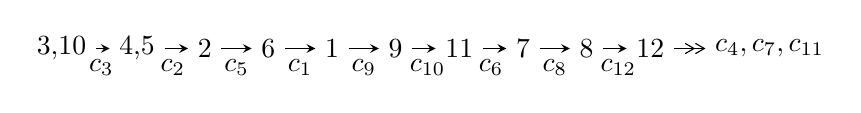
\begin{tikzpicture}[x=23pt, y=7pt]
	% node
	\node (A0) at (-1/8, 0) {3,10};
	\node (A1) at (17/16, 0) {4,5};
	\node (A2) at (17/8, 0) {2};
	\node (A3) at (25/8, 0) {6};
	\node (A4) at (33/8, 0) {1};
	\node (A5) at (41/8, 0) {9};
	\node (A6) at (49/8, 0) {11};
	\node (A7) at (57/8, 0) {7};
	\node (A8) at (65/8, 0) {8};
	\node (A9) at (73/8, 0) {12};
	\node (C1) at (1/2, -1) {$c_{3}$};
	\node (C2) at (13/8, -1) {$c_{2}$};
	\node (C3) at (21/8, -1) {$c_{5}$};
	\node (C4) at (29/8, -1) {$c_{1}$};
	\node (C5) at (37/8, -1) {$c_{9}$};
	\node (C6) at (45/8, -1) {$c_{10}$};
	\node (C7) at (53/8, -1) {$c_{6}$};
	\node (C8) at (61/8, -1) {$c_{8}$};
	\node (C9) at (69/8, -1) {$c_{12}$};
	\node (A10) at (11, 0) {$c_{4},c_{7},c_{11}$};

	% edge
	\draw[->,>=stealth]	
	(A0) edge (A1) (A1) edge (A2) (A2) edge (A3) (A3) edge (A4) (A4) edge (A5) (A5) edge (A6) (A6) edge (A7) (A7) edge (A8) (A8) edge (A9) ;
	\draw[->>,>={angle 60}]	
	(A9) edge (A10);
\end{tikzpicture} \\ 

\end{tabular} \\

\footnotetext{
The image of knot diagram is generated by the software ``\textbf{Draw programme}" developed by Andrew Bartholomew(\url{http://www.layer8.co.uk/maths/draw/index.htm\#Running-draw}), where we modified some parts for our purpose(\url{https://github.com/CATsTAILs/LinksPainter}).
}\phantom \\ \newline 
\centering \textbf{Ideals for irreducible components\footnotemark of $X_{\text{par}}$} 
 
\begin{align*}
I^u_{1}&=\langle 
1.76155\times10^{30} u^{55}+2.38665\times10^{30} u^{54}+\cdots+1.86805\times10^{31} b-5.18520\times10^{31},\\
\phantom{I^u_{1}}&\phantom{= \langle  }7.54734\times10^{30} u^{55}-1.06356\times10^{31} u^{54}+\cdots+1.86805\times10^{31} a+8.01489\times10^{31},\;u^{56}- u^{55}+\cdots-44 u^2-16\rangle \\
\\
I^v_{1}&=\langle 
a,\;v^3+2 v^2+2 b+2 v+1,\;v^4+v^3+2 v^2- v+1\rangle \\
\end{align*}
\raggedright * 2 irreducible components of $\dim_{\mathbb{C}}=0$, with total 60 representations.\\
\footnotetext{All coefficients of polynomials are rational numbers. But the coefficients are sometimes approximated in decimal forms when there is not enough margin.}
\newpage
\renewcommand{\arraystretch}{1}
\centering \section*{I. $I^u_{1}= \langle 1.76\times10^{30} u^{55}+2.39\times10^{30} u^{54}+\cdots+1.87\times10^{31} b-5.19\times10^{31},\;7.55\times10^{30} u^{55}-1.06\times10^{31} u^{54}+\cdots+1.87\times10^{31} a+8.01\times10^{31},\;u^{56}- u^{55}+\cdots-44 u^2-16 \rangle$}
\flushleft \textbf{(i) Arc colorings}\\
\begin{tabular}{m{7pt} m{180pt} m{7pt} m{180pt} }
\flushright $a_{3}=$&$\begin{pmatrix}1\\0\end{pmatrix}$ \\
\flushright $a_{10}=$&$\begin{pmatrix}0\\u\end{pmatrix}$ \\
\flushright $a_{4}=$&$\begin{pmatrix}1\\u^2\end{pmatrix}$ \\
\flushright $a_{5}=$&$\begin{pmatrix}-0.404023 u^{55}+0.569343 u^{54}+\cdots+4.15487 u-4.29052\\-0.0942991 u^{55}-0.127762 u^{54}+\cdots+0.441391 u+2.77573\end{pmatrix}$ \\
\flushright $a_{2}=$&$\begin{pmatrix}-0.124417 u^{55}-0.0227610 u^{54}+\cdots+3.42223 u+3.91486\\0.197532 u^{55}-0.245618 u^{54}+\cdots+1.00380 u+1.74945\end{pmatrix}$ \\
\flushright $a_{6}=$&$\begin{pmatrix}-0.124417 u^{55}-0.0227610 u^{54}+\cdots+3.42223 u+3.91486\\-0.148908 u^{55}+0.254056 u^{54}+\cdots-2.99446 u-4.10429\end{pmatrix}$ \\
\flushright $a_{1}=$&$\begin{pmatrix}0.0731156 u^{55}-0.268379 u^{54}+\cdots+4.42602 u+5.66431\\0.197532 u^{55}-0.245618 u^{54}+\cdots+1.00380 u+1.74945\end{pmatrix}$ \\
\flushright $a_{9}=$&$\begin{pmatrix}u\\u^3+u\end{pmatrix}$ \\
\flushright $a_{11}=$&$\begin{pmatrix}u^3\\u^5+u^3+u\end{pmatrix}$ \\
\flushright $a_{7}=$&$\begin{pmatrix}0.113306 u^{55}+0.203193 u^{54}+\cdots-3.36863 u-1.54199\\-0.262328 u^{55}+0.0564765 u^{54}+\cdots+0.999404 u+0.529453\end{pmatrix}$ \\
\flushright $a_{8}=$&$\begin{pmatrix}-0.516553 u^{55}+0.486410 u^{54}+\cdots+8.01784 u-2.62530\\-0.254069 u^{55}+0.475756 u^{54}+\cdots+2.22140 u-6.56977\end{pmatrix}$ \\
\flushright $a_{12}=$&$\begin{pmatrix}0.330162 u^{55}+0.368862 u^{54}+\cdots-9.49132 u-8.58801\\-0.363570 u^{55}+0.132323 u^{54}+\cdots+7.63673 u+0.248734\end{pmatrix}$\\&\end{tabular}
\flushleft \textbf{(ii) Obstruction class $= -1$}\\~\\
\flushleft \textbf{(iii) Cusp Shapes $= -0.0743933 u^{55}-0.650973 u^{54}+\cdots-12.4637 u+17.4604$}\\~\\
\newpage\renewcommand{\arraystretch}{1}
\flushleft \textbf{(iv) u-Polynomials at the component}\newline \\
\begin{tabular}{m{50pt}|m{274pt}}
Crossings & \hspace{64pt}u-Polynomials at each crossing \\
\hline $$\begin{aligned}c_{1},c_{4}\end{aligned}$$&$\begin{aligned}
&u^{56}+19 u^{55}+\cdots-20 u+1
\end{aligned}$\\
\hline $$\begin{aligned}c_{2},c_{5}\end{aligned}$$&$\begin{aligned}
&u^{56}+3 u^{55}+\cdots+2 u+1
\end{aligned}$\\
\hline $$\begin{aligned}c_{3},c_{9}\end{aligned}$$&$\begin{aligned}
&u^{56}- u^{55}+\cdots-44 u^2-16
\end{aligned}$\\
\hline $$\begin{aligned}c_{6},c_{7},c_{8}\\c_{11},c_{12}\end{aligned}$$&$\begin{aligned}
&u^{56}-3 u^{55}+\cdots+2 u-1
\end{aligned}$\\
\hline $$\begin{aligned}c_{10}\end{aligned}$$&$\begin{aligned}
&u^{56}-25 u^{55}+\cdots-1408 u+256
\end{aligned}$\\
\hline
\end{tabular}\\~\\
\newpage\renewcommand{\arraystretch}{1}
\flushleft \textbf{(v) Riley Polynomials at the component}\newline \\
\begin{tabular}{m{50pt}|m{274pt}}
Crossings & \hspace{64pt}Riley Polynomials at each crossing \\
\hline $$\begin{aligned}c_{1},c_{4}\end{aligned}$$&$\begin{aligned}
&y^{56}+39 y^{55}+\cdots-388 y+1
\end{aligned}$\\
\hline $$\begin{aligned}c_{2},c_{5}\end{aligned}$$&$\begin{aligned}
&y^{56}+19 y^{55}+\cdots-20 y+1
\end{aligned}$\\
\hline $$\begin{aligned}c_{3},c_{9}\end{aligned}$$&$\begin{aligned}
&y^{56}+25 y^{55}+\cdots+1408 y+256
\end{aligned}$\\
\hline $$\begin{aligned}c_{6},c_{7},c_{8}\\c_{11},c_{12}\end{aligned}$$&$\begin{aligned}
&y^{56}-73 y^{55}+\cdots+16 y+1
\end{aligned}$\\
\hline $$\begin{aligned}c_{10}\end{aligned}$$&$\begin{aligned}
&y^{56}+5 y^{55}+\cdots-925696 y+65536
\end{aligned}$\\
\hline
\end{tabular}\\~\\
\newpage\flushleft \textbf{(vi) Complex Volumes and Cusp Shapes}
$$\begin{array}{c|c|c}  
\text{Solutions to }I^u_{1}& \I (\text{vol} + \sqrt{-1}CS) & \text{Cusp shape}\\
 \hline 
\begin{aligned}
u &= \phantom{-}0.945963 + 0.329000 I \\
a &= \phantom{-}0.700162 + 0.301248 I \\
b &= -0.710485 + 0.729480 I\end{aligned}
 & \phantom{-}3.41470 + 0.08627 I & \phantom{-}10.40732 - 0.41249 I \\ \hline\begin{aligned}
u &= \phantom{-}0.945963 - 0.329000 I \\
a &= \phantom{-}0.700162 - 0.301248 I \\
b &= -0.710485 - 0.729480 I\end{aligned}
 & \phantom{-}3.41470 - 0.08627 I & \phantom{-}10.40732 + 0.41249 I \\ \hline\begin{aligned}
u &= \phantom{-}0.625712 + 0.814457 I \\
a &= \phantom{-}0.889757 + 0.875058 I \\
b &= -0.083216 + 1.022700 I\end{aligned}
 & -3.46331 - 2.44033 I & -1.79100 + 4.21493 I \\ \hline\begin{aligned}
u &= \phantom{-}0.625712 - 0.814457 I \\
a &= \phantom{-}0.889757 - 0.875058 I \\
b &= -0.083216 - 1.022700 I\end{aligned}
 & -3.46331 + 2.44033 I & -1.79100 - 4.21493 I \\ \hline\begin{aligned}
u &= \phantom{-}0.323104 + 1.005060 I \\
a &= \phantom{-}0.642445 - 0.528510 I \\
b &= -0.489124 - 1.083120 I\end{aligned}
 & \phantom{-}10.64430 + 0.45572 I & \phantom{-}9.98152 - 0.50436 I \\ \hline\begin{aligned}
u &= \phantom{-}0.323104 - 1.005060 I \\
a &= \phantom{-}0.642445 + 0.528510 I \\
b &= -0.489124 + 1.083120 I\end{aligned}
 & \phantom{-}10.64430 - 0.45572 I & \phantom{-}9.98152 + 0.50436 I \\ \hline\begin{aligned}
u &= \phantom{-}0.371261 + 0.991405 I \\
a &= \phantom{-}0.781690 + 0.096007 I \\
b &= -0.675087 + 0.237892 I\end{aligned}
 & \phantom{-}3.78611 - 2.97347 I & \phantom{-}12.77186 + 5.12067 I \\ \hline\begin{aligned}
u &= \phantom{-}0.371261 - 0.991405 I \\
a &= \phantom{-}0.781690 - 0.096007 I \\
b &= -0.675087 - 0.237892 I\end{aligned}
 & \phantom{-}3.78611 + 2.97347 I & \phantom{-}12.77186 - 5.12067 I \\ \hline\begin{aligned}
u &= \phantom{-}0.284163 + 1.021260 I \\
a &= -1.11146 - 1.51595 I \\
b &= \phantom{-}0.733335 + 0.752099 I\end{aligned}
 & \phantom{-}3.44212 + 1.17546 I & \phantom{-}10.25427 - 3.27090 I \\ \hline\begin{aligned}
u &= \phantom{-}0.284163 - 1.021260 I \\
a &= -1.11146 + 1.51595 I \\
b &= \phantom{-}0.733335 - 0.752099 I\end{aligned}
 & \phantom{-}3.44212 - 1.17546 I & \phantom{-}10.25427 + 3.27090 I\\
 \hline 
 \end{array}$$\newpage$$\begin{array}{c|c|c}  
\text{Solutions to }I^u_{1}& \I (\text{vol} + \sqrt{-1}CS) & \text{Cusp shape}\\
 \hline 
\begin{aligned}
u &= -0.661266 + 0.661352 I \\
a &= \phantom{-}1.09003 - 0.94478 I \\
b &= -0.000047 - 0.953461 I\end{aligned}
 & -1.41938 - 0.49911 I & \phantom{-}2.60701 + 1.40158 I \\ \hline\begin{aligned}
u &= -0.661266 - 0.661352 I \\
a &= \phantom{-}1.09003 + 0.94478 I \\
b &= -0.000047 + 0.953461 I\end{aligned}
 & -1.41938 + 0.49911 I & \phantom{-}2.60701 - 1.40158 I \\ \hline\begin{aligned}
u &= -0.978145 + 0.449475 I \\
a &= \phantom{-}0.635866 + 0.398468 I \\
b &= -0.681700 + 0.964218 I\end{aligned}
 & \phantom{-}2.70209 - 5.44166 I & \phantom{-}8.56320 + 6.09737 I \\ \hline\begin{aligned}
u &= -0.978145 - 0.449475 I \\
a &= \phantom{-}0.635866 - 0.398468 I \\
b &= -0.681700 - 0.964218 I\end{aligned}
 & \phantom{-}2.70209 + 5.44166 I & \phantom{-}8.56320 - 6.09737 I \\ \hline\begin{aligned}
u &= \phantom{-}0.739636 + 0.543266 I \\
a &= \phantom{-}1.27278 + 1.20579 I \\
b &= \phantom{-}0.109646 + 0.952563 I\end{aligned}
 & \phantom{-}6.95218 + 1.78242 I & \phantom{-}3.71796 - 0.00626 I \\ \hline\begin{aligned}
u &= \phantom{-}0.739636 - 0.543266 I \\
a &= \phantom{-}1.27278 - 1.20579 I \\
b &= \phantom{-}0.109646 - 0.952563 I\end{aligned}
 & \phantom{-}6.95218 - 1.78242 I & \phantom{-}3.71796 + 0.00626 I \\ \hline\begin{aligned}
u &= -0.423575 + 1.030690 I \\
a &= -2.51731 + 0.08098 I \\
b &= \phantom{-}0.696401 + 0.959847 I\end{aligned}
 & \phantom{-}2.80455 + 4.29067 I & \phantom{-}8.68297 - 2.64204 I \\ \hline\begin{aligned}
u &= -0.423575 - 1.030690 I \\
a &= -2.51731 - 0.08098 I \\
b &= \phantom{-}0.696401 - 0.959847 I\end{aligned}
 & \phantom{-}2.80455 - 4.29067 I & \phantom{-}8.68297 + 2.64204 I \\ \hline\begin{aligned}
u &= \phantom{-}0.144714 + 0.863875 I \\
a &= -3.05379 + 1.22740 I \\
b &= \phantom{-}0.662709 - 0.878637 I\end{aligned}
 & \phantom{-}9.78220 - 2.56986 I & \phantom{-}13.5531 + 4.3615 I \\ \hline\begin{aligned}
u &= \phantom{-}0.144714 - 0.863875 I \\
a &= -3.05379 - 1.22740 I \\
b &= \phantom{-}0.662709 + 0.878637 I\end{aligned}
 & \phantom{-}9.78220 + 2.56986 I & \phantom{-}13.5531 - 4.3615 I\\
 \hline 
 \end{array}$$\newpage$$\begin{array}{c|c|c}  
\text{Solutions to }I^u_{1}& \I (\text{vol} + \sqrt{-1}CS) & \text{Cusp shape}\\
 \hline 
\begin{aligned}
u &= -0.588153 + 0.958301 I \\
a &= \phantom{-}0.773912 - 0.833223 I \\
b &= -0.137469 - 1.083360 I\end{aligned}
 & -0.51184 + 5.35586 I & \phantom{-}4.95676 - 7.14944 I \\ \hline\begin{aligned}
u &= -0.588153 - 0.958301 I \\
a &= \phantom{-}0.773912 + 0.833223 I \\
b &= -0.137469 + 1.083360 I\end{aligned}
 & -0.51184 - 5.35586 I & \phantom{-}4.95676 + 7.14944 I \\ \hline\begin{aligned}
u &= -0.473668 + 1.064350 I \\
a &= -0.68920 + 1.25309 I \\
b &= \phantom{-}0.770337 - 0.690812 I\end{aligned}
 & \phantom{-}2.37111 + 2.38012 I & \phantom{-}7.11781 - 3.12902 I \\ \hline\begin{aligned}
u &= -0.473668 - 1.064350 I \\
a &= -0.68920 - 1.25309 I \\
b &= \phantom{-}0.770337 + 0.690812 I\end{aligned}
 & \phantom{-}2.37111 - 2.38012 I & \phantom{-}7.11781 + 3.12902 I \\ \hline\begin{aligned}
u &= -0.306607 + 0.768934 I \\
a &= \phantom{-}0.677930 + 0.501746 I \\
b &= -0.495582 + 1.016170 I\end{aligned}
 & \phantom{-}1.59907 - 1.22012 I & \phantom{-}10.24669 - 1.76763 I \\ \hline\begin{aligned}
u &= -0.306607 - 0.768934 I \\
a &= \phantom{-}0.677930 - 0.501746 I \\
b &= -0.495582 - 1.016170 I\end{aligned}
 & \phantom{-}1.59907 + 1.22012 I & \phantom{-}10.24669 + 1.76763 I \\ \hline\begin{aligned}
u &= \phantom{-}0.691853 + 0.442021 I \\
a &= \phantom{-}0.666356 - 0.423245 I \\
b &= -0.608819 - 0.951542 I\end{aligned}
 & -0.47690 + 3.08931 I & \phantom{-}0.47513 - 3.63327 I \\ \hline\begin{aligned}
u &= \phantom{-}0.691853 - 0.442021 I \\
a &= \phantom{-}0.666356 + 0.423245 I \\
b &= -0.608819 + 0.951542 I\end{aligned}
 & -0.47690 - 3.08931 I & \phantom{-}0.47513 + 3.63327 I \\ \hline\begin{aligned}
u &= -1.123100 + 0.376086 I \\
a &= \phantom{-}0.673422 - 0.285619 I \\
b &= -0.777518 - 0.731848 I\end{aligned}
 & \phantom{-}12.79390 - 1.04374 I & \phantom{-}11.13568 + 0. I\phantom{ +0.000000I} \\ \hline\begin{aligned}
u &= -1.123100 - 0.376086 I \\
a &= \phantom{-}0.673422 + 0.285619 I \\
b &= -0.777518 + 0.731848 I\end{aligned}
 & \phantom{-}12.79390 + 1.04374 I & \phantom{-}11.13568 + 0. I\phantom{ +0.000000I}\\
 \hline 
 \end{array}$$\newpage$$\begin{array}{c|c|c}  
\text{Solutions to }I^u_{1}& \I (\text{vol} + \sqrt{-1}CS) & \text{Cusp shape}\\
 \hline 
\begin{aligned}
u &= \phantom{-}0.031496 + 1.220130 I \\
a &= -1.73190 + 0.77105 I \\
b &= \phantom{-}0.769526 - 0.864952 I\end{aligned}
 & \phantom{-}9.36102 - 2.89044 I & \phantom{-}13.8461 + 3.0592 I \\ \hline\begin{aligned}
u &= \phantom{-}0.031496 - 1.220130 I \\
a &= -1.73190 - 0.77105 I \\
b &= \phantom{-}0.769526 + 0.864952 I\end{aligned}
 & \phantom{-}9.36102 + 2.89044 I & \phantom{-}13.8461 - 3.0592 I \\ \hline\begin{aligned}
u &= \phantom{-}0.568066 + 1.084730 I \\
a &= -2.24565 - 0.41344 I \\
b &= \phantom{-}0.703592 - 0.999172 I\end{aligned}
 & \phantom{-}1.44085 - 7.97313 I & \phantom{-0.000000 -}0. + 7.82699 I \\ \hline\begin{aligned}
u &= \phantom{-}0.568066 - 1.084730 I \\
a &= -2.24565 + 0.41344 I \\
b &= \phantom{-}0.703592 + 0.999172 I\end{aligned}
 & \phantom{-}1.44085 + 7.97313 I & \phantom{-0.000000 } 0. - 7.82699 I \\ \hline\begin{aligned}
u &= \phantom{-}0.591719 + 1.074220 I \\
a &= \phantom{-}0.704304 + 0.824413 I \\
b &= -0.157829 + 1.132950 I\end{aligned}
 & \phantom{-}8.62037 - 6.88650 I & \phantom{-0.000000 } 0 \\ \hline\begin{aligned}
u &= \phantom{-}0.591719 - 1.074220 I \\
a &= \phantom{-}0.704304 - 0.824413 I \\
b &= -0.157829 - 1.132950 I\end{aligned}
 & \phantom{-}8.62037 + 6.88650 I & \phantom{-0.000000 } 0 \\ \hline\begin{aligned}
u &= -0.422992 + 1.152020 I \\
a &= \phantom{-}0.742663 - 0.089155 I \\
b &= -0.772781 - 0.231893 I\end{aligned}
 & \phantom{-}13.22670 + 4.07484 I & \phantom{-}13.16985 + 0. I\phantom{ +0.000000I} \\ \hline\begin{aligned}
u &= -0.422992 - 1.152020 I \\
a &= \phantom{-}0.742663 + 0.089155 I \\
b &= -0.772781 + 0.231893 I\end{aligned}
 & \phantom{-}13.22670 - 4.07484 I & \phantom{-}13.16985 + 0. I\phantom{ +0.000000I} \\ \hline\begin{aligned}
u &= \phantom{-}1.127950 + 0.485672 I \\
a &= \phantom{-}0.618155 - 0.389809 I \\
b &= -0.718412 - 0.980360 I\end{aligned}
 & \phantom{-}12.03690 + 6.70540 I & \phantom{-0.000000 } 0 \\ \hline\begin{aligned}
u &= \phantom{-}1.127950 - 0.485672 I \\
a &= \phantom{-}0.618155 + 0.389809 I \\
b &= -0.718412 + 0.980360 I\end{aligned}
 & \phantom{-}12.03690 - 6.70540 I & \phantom{-0.000000 } 0\\
 \hline 
 \end{array}$$\newpage$$\begin{array}{c|c|c}  
\text{Solutions to }I^u_{1}& \I (\text{vol} + \sqrt{-1}CS) & \text{Cusp shape}\\
 \hline 
\begin{aligned}
u &= -0.754125\phantom{ +0.000000I} \\
a &= \phantom{-}0.724705\phantom{ +0.000000I} \\
b &= \phantom{-}0.455004\phantom{ +0.000000I}\end{aligned}
 & \phantom{-}9.83456\phantom{ +0.000000I} & \phantom{-}8.53390\phantom{ +0.000000I} \\ \hline\begin{aligned}
u &= -0.256062 + 0.665128 I \\
a &= \phantom{-}0.904103 - 0.096717 I \\
b &= -0.397261 - 0.233187 I\end{aligned}
 & \phantom{-}0.338686 + 0.999830 I & \phantom{-}6.13657 - 6.36197 I \\ \hline\begin{aligned}
u &= -0.256062 - 0.665128 I \\
a &= \phantom{-}0.904103 + 0.096717 I \\
b &= -0.397261 + 0.233187 I\end{aligned}
 & \phantom{-}0.338686 - 0.999830 I & \phantom{-}6.13657 + 6.36197 I \\ \hline\begin{aligned}
u &= \phantom{-}0.588126 + 1.170640 I \\
a &= -0.617779 - 0.984152 I \\
b &= \phantom{-}0.824403 + 0.669190 I\end{aligned}
 & \phantom{-}6.05580 - 5.59891 I & \phantom{-0.000000 } 0 \\ \hline\begin{aligned}
u &= \phantom{-}0.588126 - 1.170640 I \\
a &= -0.617779 + 0.984152 I \\
b &= \phantom{-}0.824403 - 0.669190 I\end{aligned}
 & \phantom{-}6.05580 + 5.59891 I & \phantom{-0.000000 } 0 \\ \hline\begin{aligned}
u &= -0.658056 + 1.167570 I \\
a &= -1.99266 + 0.49709 I \\
b &= \phantom{-}0.720138 + 1.025440 I\end{aligned}
 & \phantom{-}4.97425 + 11.38970 I & \phantom{-0.000000 } 0 \\ \hline\begin{aligned}
u &= -0.658056 - 1.167570 I \\
a &= -1.99266 - 0.49709 I \\
b &= \phantom{-}0.720138 - 1.025440 I\end{aligned}
 & \phantom{-}4.97425 - 11.38970 I & \phantom{-0.000000 } 0 \\ \hline\begin{aligned}
u &= -0.66401 + 1.25051 I \\
a &= -0.594793 + 0.840724 I \\
b &= \phantom{-}0.862806 - 0.659902 I\end{aligned}
 & \phantom{-}15.6301 + 7.4127 I & \phantom{-0.000000 } 0 \\ \hline\begin{aligned}
u &= -0.66401 - 1.25051 I \\
a &= -0.594793 - 0.840724 I \\
b &= \phantom{-}0.862806 + 0.659902 I\end{aligned}
 & \phantom{-}15.6301 - 7.4127 I & \phantom{-0.000000 } 0 \\ \hline\begin{aligned}
u &= \phantom{-}0.72488 + 1.23003 I \\
a &= -1.83482 - 0.53507 I \\
b &= \phantom{-}0.732388 - 1.044730 I\end{aligned}
 & \phantom{-}14.4517 - 13.3499 I & \phantom{-0.000000 } 0\\
 \hline 
 \end{array}$$\newpage$$\begin{array}{c|c|c}  
\text{Solutions to }I^u_{1}& \I (\text{vol} + \sqrt{-1}CS) & \text{Cusp shape}\\
 \hline 
\begin{aligned}
u &= \phantom{-}0.72488 - 1.23003 I \\
a &= -1.83482 + 0.53507 I \\
b &= \phantom{-}0.732388 + 1.044730 I\end{aligned}
 & \phantom{-}14.4517 + 13.3499 I & \phantom{-0.000000 } 0 \\ \hline\begin{aligned}
u &= -0.520003 + 0.233894 I \\
a &= \phantom{-}0.762531 - 0.369226 I \\
b &= -0.544789 - 0.773570 I\end{aligned}
 & \phantom{-}0.16754 + 1.55102 I & -0.50728 - 2.39456 I \\ \hline\begin{aligned}
u &= -0.520003 - 0.233894 I \\
a &= \phantom{-}0.762531 + 0.369226 I \\
b &= -0.544789 + 0.773570 I\end{aligned}
 & \phantom{-}0.16754 - 1.55102 I & -0.50728 + 2.39456 I \\ \hline\begin{aligned}
u &= -0.04885 + 1.43050 I \\
a &= -1.47868 - 0.48254 I \\
b &= \phantom{-}0.825254 + 0.886448 I\end{aligned}
 & -19.6229 + 3.0661 I & \phantom{-0.000000 } 0 \\ \hline\begin{aligned}
u &= -0.04885 - 1.43050 I \\
a &= -1.47868 + 0.48254 I \\
b &= \phantom{-}0.825254 - 0.886448 I\end{aligned}
 & -19.6229 - 3.0661 I & \phantom{-0.000000 } 0 \\ \hline\begin{aligned}
u &= \phantom{-}0.485800\phantom{ +0.000000I} \\
a &= \phantom{-}0.939168\phantom{ +0.000000I} \\
b &= \phantom{-}0.224170\phantom{ +0.000000I}\end{aligned}
 & \phantom{-}1.28164\phantom{ +0.000000I} & \phantom{-}7.41160\phantom{ +0.000000I}\\
 \hline 
 \end{array}$$\newpage\newpage\renewcommand{\arraystretch}{1}
\centering \section*{II. $I^v_{1}= \langle a,\;v^3+2 v^2+2 b+2 v+1,\;v^4+v^3+2 v^2- v+1 \rangle$}
\flushleft \textbf{(i) Arc colorings}\\
\begin{tabular}{m{7pt} m{180pt} m{7pt} m{180pt} }
\flushright $a_{3}=$&$\begin{pmatrix}1\\0\end{pmatrix}$ \\
\flushright $a_{10}=$&$\begin{pmatrix}v\\0\end{pmatrix}$ \\
\flushright $a_{4}=$&$\begin{pmatrix}1\\0\end{pmatrix}$ \\
\flushright $a_{5}=$&$\begin{pmatrix}0\\-\frac{1}{2} v^3- v^2- v-\frac{1}{2}\end{pmatrix}$ \\
\flushright $a_{2}=$&$\begin{pmatrix}1\\\frac{1}{2} v^3+v^2+v-\frac{1}{2}\end{pmatrix}$ \\
\flushright $a_{6}=$&$\begin{pmatrix}-\frac{1}{2} v^3- v^2- v-\frac{1}{2}\\-\frac{1}{2} v^3- v^2- v+\frac{1}{2}\end{pmatrix}$ \\
\flushright $a_{1}=$&$\begin{pmatrix}\frac{1}{2} v^3+v^2+v+\frac{1}{2}\\\frac{1}{2} v^3+v^2+v-\frac{1}{2}\end{pmatrix}$ \\
\flushright $a_{9}=$&$\begin{pmatrix}v\\0\end{pmatrix}$ \\
\flushright $a_{11}=$&$\begin{pmatrix}v\\0\end{pmatrix}$ \\
\flushright $a_{7}=$&$\begin{pmatrix}- v\\-\frac{1}{2} v^3- v^2- v+\frac{1}{2}\end{pmatrix}$ \\
\flushright $a_{8}=$&$\begin{pmatrix}0\\-\frac{1}{2} v^3- v+\frac{1}{2}\end{pmatrix}$ \\
\flushright $a_{12}=$&$\begin{pmatrix}\frac{1}{2} v^3+v^2+v+\frac{1}{2}\\\frac{1}{2} v^3+v-\frac{1}{2}\end{pmatrix}$\\&\end{tabular}
\flushleft \textbf{(ii) Obstruction class $= 1$}\\~\\
\flushleft \textbf{(iii) Cusp Shapes $= -3 v^3-5 v^2-7 v+7$}\\~\\
\newpage\renewcommand{\arraystretch}{1}
\flushleft \textbf{(iv) u-Polynomials at the component}\newline \\
\begin{tabular}{m{50pt}|m{274pt}}
Crossings & \hspace{64pt}u-Polynomials at each crossing \\
\hline $$\begin{aligned}c_{1},c_{4},c_{5}\end{aligned}$$&$\begin{aligned}
&(u^2- u+1)^2
\end{aligned}$\\
\hline $$\begin{aligned}c_{2}\end{aligned}$$&$\begin{aligned}
&(u^2+u+1)^2
\end{aligned}$\\
\hline $$\begin{aligned}c_{3},c_{9},c_{10}\end{aligned}$$&$\begin{aligned}
&u^4
\end{aligned}$\\
\hline $$\begin{aligned}c_{6},c_{7},c_{8}\end{aligned}$$&$\begin{aligned}
&(u^2- u-1)^2
\end{aligned}$\\
\hline $$\begin{aligned}c_{11},c_{12}\end{aligned}$$&$\begin{aligned}
&(u^2+u-1)^2
\end{aligned}$\\
\hline
\end{tabular}\\~\\
\newpage\renewcommand{\arraystretch}{1}
\flushleft \textbf{(v) Riley Polynomials at the component}\newline \\
\begin{tabular}{m{50pt}|m{274pt}}
Crossings & \hspace{64pt}Riley Polynomials at each crossing \\
\hline $$\begin{aligned}c_{1},c_{2},c_{4}\\c_{5}\end{aligned}$$&$\begin{aligned}
&(y^2+y+1)^2
\end{aligned}$\\
\hline $$\begin{aligned}c_{3},c_{9},c_{10}\end{aligned}$$&$\begin{aligned}
&y^4
\end{aligned}$\\
\hline $$\begin{aligned}c_{6},c_{7},c_{8}\\c_{11},c_{12}\end{aligned}$$&$\begin{aligned}
&(y^2-3 y+1)^2
\end{aligned}$\\
\hline
\end{tabular}\\~\\
\newpage\flushleft \textbf{(vi) Complex Volumes and Cusp Shapes}
$$\begin{array}{c|c|c}  
\text{Solutions to }I^v_{1}& \I (\text{vol} + \sqrt{-1}CS) & \text{Cusp shape}\\
 \hline 
\begin{aligned}
v &= \phantom{-}0.309017 + 0.535233 I \\
a &= \phantom{-0.000000 } 0 \\
b &= -0.500000 - 0.866025 I\end{aligned}
 & \phantom{-}0.98696 + 2.02988 I & \phantom{-}6.50000 - 5.40059 I \\ \hline\begin{aligned}
v &= \phantom{-}0.309017 - 0.535233 I \\
a &= \phantom{-0.000000 } 0 \\
b &= -0.500000 + 0.866025 I\end{aligned}
 & \phantom{-}0.98696 - 2.02988 I & \phantom{-}6.50000 + 5.40059 I \\ \hline\begin{aligned}
v &= -0.80902 + 1.40126 I \\
a &= \phantom{-0.000000 } 0 \\
b &= -0.500000 + 0.866025 I\end{aligned}
 & \phantom{-}8.88264 - 2.02988 I & \phantom{-}6.50000 + 1.52761 I \\ \hline\begin{aligned}
v &= -0.80902 - 1.40126 I \\
a &= \phantom{-0.000000 } 0 \\
b &= -0.500000 - 0.866025 I\end{aligned}
 & \phantom{-}8.88264 + 2.02988 I & \phantom{-}6.50000 - 1.52761 I\\
 \hline 
 \end{array}$$\newpage
\newpage\renewcommand{\arraystretch}{1}
\centering \section*{ III. u-Polynomials}
\begin{tabular}{m{50pt}|m{274pt}}
Crossings & \hspace{64pt}u-Polynomials at each crossing \\
\hline $$\begin{aligned}c_{1},c_{4}\end{aligned}$$&$\begin{aligned}
&((u^2- u+1)^2)(u^{56}+19 u^{55}+\cdots-20 u+1)
\end{aligned}$\\
\hline $$\begin{aligned}c_{2}\end{aligned}$$&$\begin{aligned}
&((u^2+u+1)^2)(u^{56}+3 u^{55}+\cdots+2 u+1)
\end{aligned}$\\
\hline $$\begin{aligned}c_{3},c_{9}\end{aligned}$$&$\begin{aligned}
&u^4(u^{56}- u^{55}+\cdots-44 u^2-16)
\end{aligned}$\\
\hline $$\begin{aligned}c_{5}\end{aligned}$$&$\begin{aligned}
&((u^2- u+1)^2)(u^{56}+3 u^{55}+\cdots+2 u+1)
\end{aligned}$\\
\hline $$\begin{aligned}c_{6},c_{7},c_{8}\end{aligned}$$&$\begin{aligned}
&((u^2- u-1)^2)(u^{56}-3 u^{55}+\cdots+2 u-1)
\end{aligned}$\\
\hline $$\begin{aligned}c_{10}\end{aligned}$$&$\begin{aligned}
&u^4(u^{56}-25 u^{55}+\cdots-1408 u+256)
\end{aligned}$\\
\hline $$\begin{aligned}c_{11},c_{12}\end{aligned}$$&$\begin{aligned}
&((u^2+u-1)^2)(u^{56}-3 u^{55}+\cdots+2 u-1)
\end{aligned}$\\
\hline
\end{tabular}\newpage\renewcommand{\arraystretch}{1}
\centering \section*{ IV. Riley Polynomials}
\begin{tabular}{m{50pt}|m{274pt}}
Crossings & \hspace{64pt}Riley Polynomials at each crossing \\
\hline $$\begin{aligned}c_{1},c_{4}\end{aligned}$$&$\begin{aligned}
&((y^2+y+1)^2)(y^{56}+39 y^{55}+\cdots-388 y+1)
\end{aligned}$\\
\hline $$\begin{aligned}c_{2},c_{5}\end{aligned}$$&$\begin{aligned}
&((y^2+y+1)^2)(y^{56}+19 y^{55}+\cdots-20 y+1)
\end{aligned}$\\
\hline $$\begin{aligned}c_{3},c_{9}\end{aligned}$$&$\begin{aligned}
&y^4(y^{56}+25 y^{55}+\cdots+1408 y+256)
\end{aligned}$\\
\hline $$\begin{aligned}c_{6},c_{7},c_{8}\\c_{11},c_{12}\end{aligned}$$&$\begin{aligned}
&((y^2-3 y+1)^2)(y^{56}-73 y^{55}+\cdots+16 y+1)
\end{aligned}$\\
\hline $$\begin{aligned}c_{10}\end{aligned}$$&$\begin{aligned}
&y^4(y^{56}+5 y^{55}+\cdots-925696 y+65536)
\end{aligned}$\\
\hline
\end{tabular}
\vskip 2pc
\end{document}